% !TeX root = ../main.tex
\chapter{Unidad 10: El ruido y su caracterización}

\section*{Objetivo pedagógico}
\noindent\textbf{Objetivo.} Comprender los tipos de ruido, sus características espectrales y temporales, sus efectos en la salud auditiva y no auditiva, y las técnicas de medición, enmascaramiento y control, aplicándolos a la fonoaudiología (como en audiometrías y terapias para tinnitus) y al diseño de entornos clínicos. Se incluyen ejemplos clínicos, actividades prácticas, recursos multimedia y ejercicios de autoevaluación.

\noindent\textbf{Pregunta inicial.} ¿Por qué el ruido de una calle puede dificultar una conversación? ¿Cómo se mide y controla el ruido en una clínica? ¡Esta unidad te ayudará a entender el impacto del ruido y cómo manejarlo!

\section{Ruido versus sonido}
El \textbf{ruido} es un sonido no deseado o molesto, una percepción subjetiva. Por ejemplo, una canción puede ser música para un oyente y ruido para otro, dependiendo del contexto.

\begin{quote}
    \textbf{Ejemplo clínico.} En una cabina audiométrica, el ruido de un ventilador ($\approx$40 dBA) puede interferir con la detección de umbrales auditivos, mientras que para un paciente con tinnitus, un ruido controlado puede ser terapéutico.
\end{quote}

\section{Clasificación de los ruidos}
Los ruidos se clasifican según su duración, fuente y frecuencia:
\begin{description}
    \item[\textbf{Continuo:}] Nivel estable, como una turbina o una cascada.
    \item[\textbf{Intermitente:}] Varía con el tiempo, como el tráfico urbano.
    \item[\textbf{Impulsivo:}] Picos breves ($<$1 s), como un martillazo o disparo, medidos con $L_{\text{peak}}$.
    \item[\textbf{Ambiental:}] Mezcla de fuentes externas (tráfico, industria, ocio).
    \item[\textbf{Industrial:}] Máquinas en fábricas, con límite de 85 dBA por 8 h.
    \item[\textbf{Impacto:}] Impulsos repetidos, como en obras o canteras.
    \item[\textbf{Baja frecuencia:}] $<$200 Hz, atraviesa paredes y causa molestias fisiológicas (por ejemplo, vibraciones).
\end{description}

\begin{quote}
    \textbf{Ejemplo clínico.} Un paciente con hipoacusia expuesto a ruido impulsivo (como martillos neumáticos) puede desarrollar un desplazamiento temporal del umbral (TTS), detectable en audiometría.
\end{quote}

\section{Ruido aleatorio y su descripción estadística}
El ruido aleatorio es impredecible y se caracteriza por:
\begin{itemize}
    \item \textbf{RMS:} Valor efectivo de la señal.
    \item \textbf{$L_{eq}$:} Nivel equivalente, promedio ponderado en el tiempo.
    \item \textbf{Percentiles:} $L_{10}$ (nivel superado el 10\% del tiempo, picos); $L_{90}$ (nivel de fondo).
\end{itemize}

\subsection{Blanco, rosa y otros espectros}
\begin{itemize}
    \item \textbf{Ruido blanco:} Energía igual por Hz, suena “siseante” (como una radio mal sintonizada).
    \item \textbf{Ruido rosa:} Energía constante por octava (–3 dB/oct), suena más equilibrado, usado en calibraciones.
    \item \textbf{Ruido vocal:} Es un ruido blanco al que se le aplica un filtro pasa-bajos con frecuencia de corte en 1000 Hz, útil en logoaudiometría.
    \item \textbf{Ruido de banda estrecha (NBN):} Ancho $\approx$1/3 de octava, usado en enmascaramiento.
\end{itemize}

\begin{quote}
    \textbf{Ejemplo clínico.} En audiometría, se usa ruido vocal para evaluar la inteligibilidad del habla, mientras que el ruido de banda estrecha enmascara el oído contralateral.
\end{quote}

\begin{figure}[h]
    \centering
    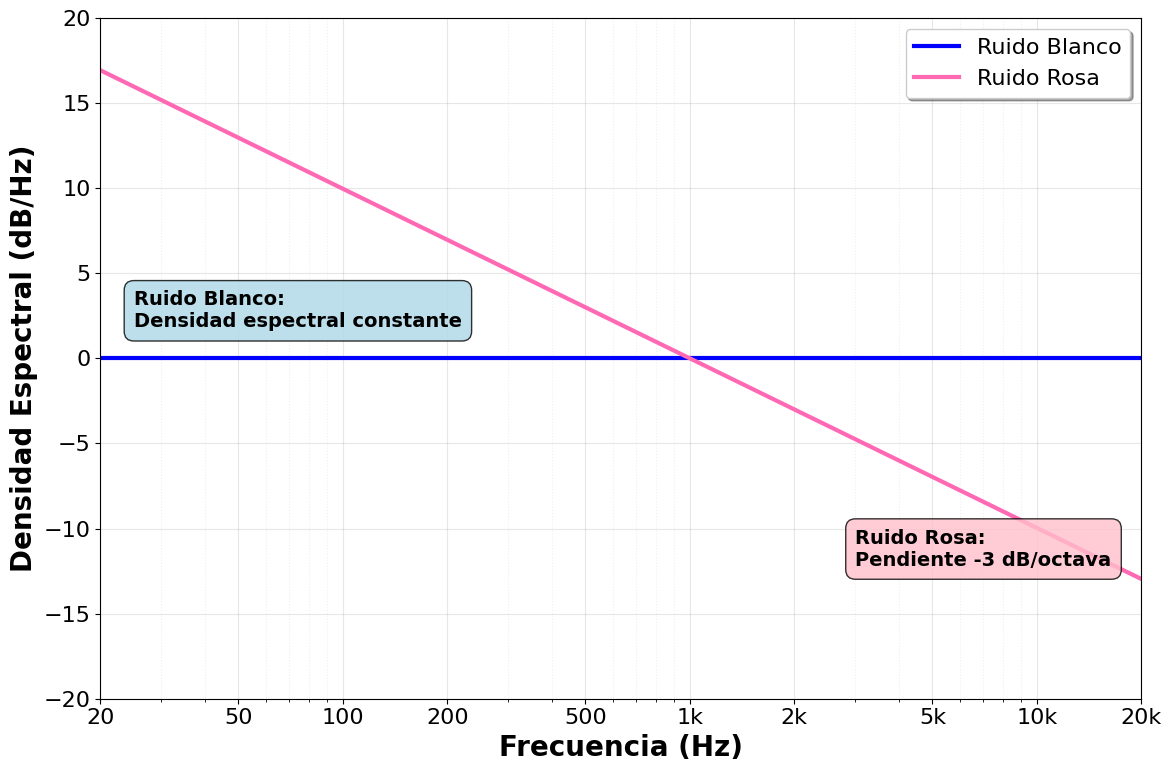
\includegraphics[width=1.0\textwidth]{figures/densidad_espectro_ruidos.png}
    \caption{Diferencias entre espectros de ruido blanco y rosa en escala logarítmica.}
    \label{densidad_espectro_ruidos}
\end{figure}


\textbf{Actividad práctica.} Usa Tone Generator (gratis) para escuchar ruido blanco y rosa. Nota cómo el ruido rosa suena más grave. Luego, graba un ruido ambiental con Audacity y observa su espectro.

\section{Técnica de enmascaramiento acústico}
El \textbf{enmascaramiento} usa ruido de banda estrecha (NBN) centrado en la frecuencia del tono a ocultar, elevando su umbral de detección. Es esencial en:
\begin{itemize}
    \item \textbf{Audiometría:} Enmascara el oído no evaluado para evitar respuestas cruzadas.
    \item \textbf{Terapia de tinnitus:} Ruido NBN a 5–10 dB sobre el tinnitus reduce su percepción.
\end{itemize}

\begin{quote}
    \textbf{Ejemplo clínico.} Para un paciente con tinnitus a 6 kHz, un audífono con NBN centrado en 6 kHz (ancho $\approx$1/3 octava) puede aliviar la molestia.
\end{quote}

\section{Efectos del ruido sobre la salud}
\begin{itemize}
    \item \textbf{Auditivos:} Pérdida auditiva inducida por ruido (NIHL, notch en 3–6 kHz), TTS, tinnitus.
    \item \textbf{No auditivos:} Estrés, insomnio, hipertensión (OMS, 2018: riesgo cardiovascular con $L_{den} > 65$ dB).
    \item \textbf{Cognitivos:} Disminución del rendimiento escolar en aulas con $L_{eq} > 65$ dB.
\end{itemize}

\begin{quote}
    \textbf{Ejemplo clínico.} Un niño en un aula ruidosa ($L_{eq} = 70$ dB) puede tener dificultades para concentrarse, afectando su aprendizaje del lenguaje.
\end{quote}

\section{Normativas y métricas}

\begin{table}[h]
    \centering
    \begin{tabular}{|l|c|c|}
        \hline
        \textbf{Entidad} & \textbf{Parámetro} & \textbf{Límite} \\
        \hline
        OMS (residencial, día) & $L_{\text{day}}$ & 55 dBA \\
        OMS (noche) & $L_{\text{night}}$ & 45 dBA \\
        ISO 1996-1/-2 & $L_{\text{den}}$ & 65 dBA \\
        OSHA (laboral) & $L_{Aeq,8h}$ & 85 dBA \\
        \hline
    \end{tabular}
    \caption{Valores guía de ruido ambiental y laboral.}
\end{table}

\subsection{Sonómetros y ponderación}
Los sonómetros clase 1 miden con ponderaciones A, C o Z y filtros temporales:
\begin{itemize}
    \item \textbf{Fast (125 ms):} Para ruidos continuos o intermitentes.
    \item \textbf{Slow (1 s):} Para promedios estables.
    \item \textbf{Impulse:} Para picos rápidos ($L_{\text{peak}}$).
\end{itemize}

\begin{quote}
    \textbf{Ejemplo clínico.} En una cabina audiométrica, un sonómetro con ponderación A verifica que el ruido de fondo sea $<$30 dBA, garantizando pruebas precisas.
\end{quote}

\section{Control y mitigación del ruido}
\begin{enumerate}
    \item \textbf{Fuente:} Silenciar máquinas, reducir velocidad, mantenimiento.
    \item \textbf{Trayecto:} Usar barreras acústicas, pantallas porosas, aislamiento (ley de masas).
    \item \textbf{Receptor:} Protectores auditivos (tapones, orejeras). Doble protección si $L_{\text{peak}} > 105$ dB.
\end{enumerate}

\begin{quote}
    \textbf{Ejemplo clínico.} En una clínica cerca de una calle ruidosa, se instalan ventanas dobles (aislamiento) y cortinas absorbentes para mantener el ruido $<$30 dBA en la cabina.
\end{quote}


\section{Ejemplos prácticos}
\begin{enumerate}
    \item \textbf{Cálculo de $L_{eq,1h}$.} Lecturas de 88, 92, 86, 90 dBA (impulsos, 15 min cada una):
    \[
    L_{eq,1h} = 10 \log_{10} \left( \frac{10^{88/10} + 10^{92/10} + 10^{86/10} + 10^{90/10}}{4} \right) \approx 89.5 \, \text{dBA}.
    \]
    \item \textbf{Atenuación de barrera.} Reducir la energía a 1/10 implica:
    \[
    \Delta L = 10 \log_{10} \left(\frac{1}{0.1}\right) = 10 \, \text{dB}.
    \]
    \item \textbf{Enmascaramiento de tinnitus.} Para 6 kHz, usar NBN centrado en 6 kHz (ancho $\approx$1/3 octava, 5–10 dB sobre el tinnitus), ajustado vía acufenometría.
\end{enumerate}

\section{Ejercicios de autoevaluación}
\begin{enumerate}
    \item Explica por qué el ruido rosa es preferido para calibrar sistemas de audio en comparación con el ruido blanco.
    \item Compara la molestia de un ruido continuo de 70 dBA con un ruido impulsivo de $L_{eq} = 55$ dBA y picos de 90 dB.
    \item Enumera tres materiales con $\alpha > 0.8$ a 1 kHz (por ejemplo, espuma acústica, cortinas gruesas, paneles perforados) y su uso en una clínica.
    \item Usa Decibel X para medir el ruido en un aula. Si $L_{eq} > 65$ dB, sugiere medidas de mitigación.
\end{enumerate}

\section{Recursos recomendados}
\begin{itemize}
    \item Video: \href{https://www.youtube.com/watch?v=Qkb2yRKJxSc&ab_channel=AudioUniversity}{``White Noise vs Pink Noise''}.
    \item App: Decibel X (gratis). Mide niveles de ruido y $L_{eq}$.
    \item App: Tone Generator (gratis). Genera ruidos blanco y rosa.
    \item Software: Room EQ Wizard (gratis). Analiza espectros y reverberación.
    \item Documento: OMS, \emph{Environmental Noise Guidelines} (2018, PDF en línea).
\end{itemize}

\section*{Glosario}
\begin{description}
    \item[\textbf{$L_{Aeq}$:}] Nivel equivalente de presión sonora ponderado A.
    \item[\textbf{$L_{\text{peak}}$:}] Nivel máximo instantáneo de un impulso.
    \item[\textbf{NBN:}] Ruido de banda estrecha, usado en enmascaramiento.
    \item[\textbf{Notch:}] Muesca en el audiograma, típica de NIHL.
\end{description}

\section*{Resumen}
\begin{itemize}
    \item \textbf{Tipos de ruido:} Continuo, intermitente, impulsivo, ambiental, baja frecuencia.
    \item \textbf{Caracterización:} Ruido blanco (plano), rosa (–3 dB/oct), vocal, NBN.
    \item \textbf{Efectos:} NIHL, tinnitus, estrés, problemas cognitivos.
    \item \textbf{Control:} Mitigación en fuente, trayecto y receptor; normativas OMS/OSHA.
\end{itemize}


\bigskip
\noindent\emph{Conclusión.} Caracterizar y controlar el ruido es clave para proteger la salud auditiva, mejorar la inteligibilidad del habla y diseñar entornos clínicos óptimos, como cabinas audiométricas. Estos conocimientos son esenciales en fonoaudiología para diagnósticos precisos y terapias efectivas, como el tratamiento del tinnitus.



%%%%%%%%%%%%%%%%%%%%%%%%%%%%%%%%%%%%%%%%%%%%%%%%%%%%%%%%%%%%%%%%%%%%%%%%%%%%%%%%%%%%%%%%%%%%%%%%%%
